% \documentclass{article}
\documentclass{report}

\usepackage{fancyhdr}
\usepackage{extramarks}
\usepackage{amsmath}
\usepackage{amsthm}
\usepackage{amsfonts}
\usepackage{tikz}
\usepackage[plain]{algorithm}
\usepackage{algpseudocode}
\usepackage{minted}
\usepackage{tcolorbox}
\newminted{python}{frame=lines,framerule=2pt}
\usepackage{graphicx}
\usepackage{enumitem}
\graphicspath{ {./images} }
\usepackage{microtype}
\usepackage{hyperref}
\usepackage{array}

\hypersetup{
    colorlinks,
    citecolor=black,
    filecolor=black,
    linkcolor=black,
    urlcolor=black
}

%
% Basic Document Settings
%

\topmargin=-0.45in
\evensidemargin=0in
\oddsidemargin=0in
\textwidth=6.5in
\textheight=9.0in
\headsep=0.25in

\linespread{1.1}

\pagestyle{fancy}
\lhead{\hmwkAuthorName}
\rhead{\hmwkClass  ~- \hmwkTitle}
\lfoot{\lastxmark}
\cfoot{\thepage}

\renewcommand\headrulewidth{0.4pt}
\renewcommand\footrulewidth{0.4pt}

\setlength\parindent{0pt}

%
% Create Problem Sections
%

\newcommand{\enterProblemHeader}[1]{
    \nobreak\extramarks{}{Problem \arabic{#1} continued on next page\ldots}\nobreak{}
    \nobreak\extramarks{Problem \arabic{#1} (continued)}{Problem \arabic{#1} continued on next page\ldots}\nobreak{}
}

\newcommand{\exitProblemHeader}[1]{
    \nobreak\extramarks{Problem \arabic{#1} (continued)}{Problem \arabic{#1} continued on next page\ldots}\nobreak{}
    \stepcounter{#1}
    \nobreak\extramarks{Problem \arabic{#1}}{}\nobreak{}
}

\setcounter{secnumdepth}{0}
\newcounter{partCounter}
\newcounter{homeworkProblemCounter}
\setcounter{homeworkProblemCounter}{1}
\nobreak\extramarks{Problem \arabic{homeworkProblemCounter}}{}\nobreak{}
\newcounter{subproblemCounter}

%
% Homework Problem Environment
%
% This environment takes an optional argument. When given, it will adjust the
% problem counter. This is useful for when the problems given for your
% assignment aren't sequential. See the last 3 problems of this template for an
% example.
%
\newenvironment{homeworkProblem}[1][-1]{
    \ifnum#1>0
        \setcounter{homeworkProblemCounter}{#1}
    \fi
    \section{Problem \arabic{homeworkProblemCounter}}
    \setcounter{partCounter}{1}
    \enterProblemHeader{homeworkProblemCounter}
}{
    \exitProblemHeader{homeworkProblemCounter}
}

%
% Homework Details
%   - Title
%   - Due date
%   - Class
%   - Section/Time
%   - Instructor
%   - Author
%

\newcommand{\hmwkTitle}{IMRT for Cancer Therapy}
\newcommand{\hmwkDueDate}{December 13, 2020}
\newcommand{\hmwkClass}{CS 5727: Optimization Methods}
\newcommand{\hmwkAuthorName}{\textbf{Shuo Han}}

%
% Title Page
%

\title{
    \vspace{2in}
    \textmd{\textbf{\hmwkClass}}\\
    \textmd{\textbf{\hmwkTitle}}\\
    \normalsize\vspace{0.1in}\small{Due: \hmwkDueDate}\\
    \vspace{3in}
}

\author{\hmwkAuthorName}
\date{}

\renewcommand{\part}[1]{\textbf{\large Part \Alph{partCounter}}\stepcounter{partCounter}\\}

\begin{document}

\maketitle

\pagebreak
\tableofcontents

\newpage


\section{1. Overview}
Intensity Modulated Radiation Therapy (IMRT) is an effective approach in cancer treatment. The main idea is to utilize beamlets to irradiate patients to kill tumor cells, while protecting healthy organs as much as possible. Therefore, the treatment plan can be formulated as an optimization problem. \\

In this project, we propose 3 radiation treatment plans. Different patients have distinct mental and physical preferences on the safety and efficiency. Doctors and patients can choose the treatment plan that is most suitable for the patient.

\section{2. Analysis}

\subsection{2.1 Classification}

Voxels on the boundaries of organs are sometimes misclassified due to the variability of the positions of patients. If tumor cells are not getting enough radiation, they might be able to grow again. To make up variations, voxels on the edge of the CTV region are classified as CTV if possible. We propose the voxel classifications in Figure 1.\\

\begin{figure}[h!]
    \centering
    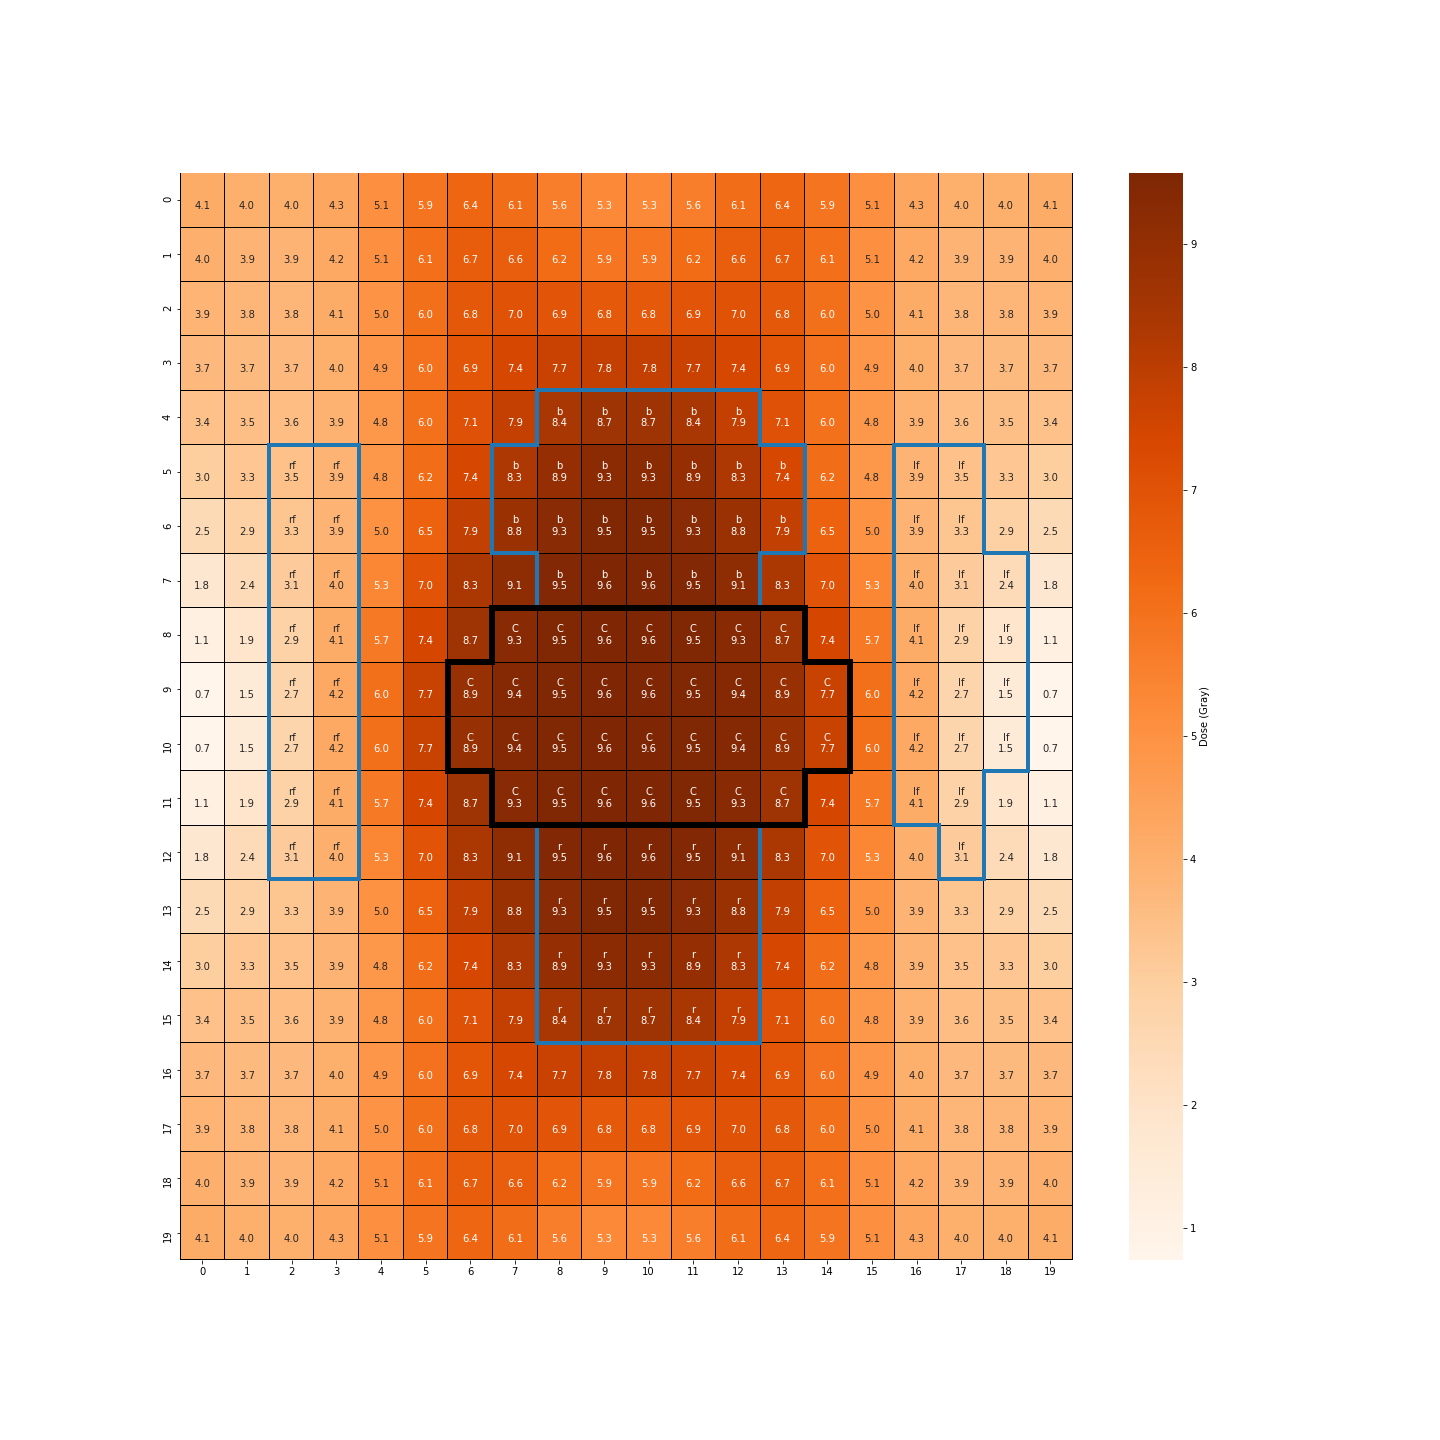
\includegraphics[width=0.95\columnwidth]{classification.png}
    \caption{Classification of Voxels}
\label{figure:1} 
\end{figure}

Figure 1 shows the classifications of 400 voxels and their doses when all beamlets have exact one intensity. The voxels in the black bounding box with letter C are considered as the CTV region. The voxels in the blue bounding boxes are Bladder (b), Rectal Solid (r), Left Femur Head (lf) and Right Femur Head (rf) respectively. Other voxels are classified as Unspecified. The color of each voxel reflects the dose received.\\

With classifications of each voxel, we are able to formulate this optimization as a mixed linear and integer programming problem.

\subsection{2.2 Formulation}
Before formulation, we declare some of the notations that will be mentioned later. For example, in the Bladder region:

\begin{itemize}
    \item $\{Bladder \}$ denotes the voxels that belong to the Bladder region.
    \item $|Bladder|$ denotes the number of voxels in the Bladder region.
\end{itemize}
\subsubsection{2.2.1 Decision Variables}

\textbf{Beamlet Intensity}\\
Intuitively, the intensities of beamlets determine the radiation doses received by all voxels. 
\begin{center}
    $x_i = \text{the intensity of beamlet i}, ~~ \forall i \in \{1, 2, \dotsc 60\}$
\end{center}

Besides, some regions have special constraints. For example, at most 10\% of the bladder should receive a dose $>$ 65.0 Gy. Those constraints introduce non-linearity and require to use binary decision variables. Therefore, we also incorporate the following decision variables in Bladder, Left Femur Head and Right Femur Head:\\


\textbf{Bladder}
\begin{center}
    $b_j= 
\begin{cases}
    0,& \text{if}~~~ D_j > 65.0\\
    1,              & D_j \leq 65.0
\end{cases} ~~~\forall j \in \{\text{Bladder}\}$\\

    $o_j = \text{the difference between the actual dose and 65.0 Gy} ~~~ \forall j \in \{\text{Bladder}\}$
\end{center}

Where:
\begin{itemize}
    \item $b_j$ denotes if the voxel has a dose no more than 65.0 Gy. if $b_j$ is 1, then the dose is less than or equal 65 Gy.
    \item $o_j$ denotes the difference between the actual dose $D_j$ and 65.0 Gy. In other words, $o_j$ is the ``overdose'' or ``underdose'' compared to 65.0 Gy.
    \item $D_j$ denotes the radiation received by voxel j. Mathematically, $o_j = D_j - 65$.
\end{itemize}

Similarly, we have decision variables for left femur head and right femur head:\\

\textbf{Left Femur Head}
\begin{center}
    $b_j= 
\begin{cases}
    0,& \text{if}~~~ D_j > 40.0\\
    1,              & D_j \leq 40.0
\end{cases} ~~~\forall j \in \{\text{Left Femur}\}$\\

    $o_j = \text{the difference between the actual dose and 40.0 Gy} ~~~ \forall j \in \{\text{Left Femur}\}$
\end{center}

\textbf{Right Femur Head}
\begin{center}
    $b_j= 
\begin{cases}
    0,& \text{if}~~~ D_j > 40.0\\
    1,              & D_j \leq 40.0
\end{cases} ~~~\forall j \in \{\text{Right Femur}\}$\\

    $o_j = \text{the difference between the actual dose and 40.0 Gy} ~~~ \forall j \in \{\text{Right Femur}\}$
\end{center}



\subsubsection{2.2.2 Objective}
The overall goal is to satisfy the constraints as much as possible. In the formulation, we can define two sets of objective.
\begin{itemize}
    \item Maximize the total doses in the CTV region, while satisfying constraints.
    \begin{center}
        $\max \sum_{j \in \{\text{CTV} \}}\sum_{i = 1}^{60} x_iw_{i,j}$
    \end{center}
    where $w_{i,j}$ denotes the dose received by voxel j from beamlet i with unit intensity. For simplicity, We denote $D_j = \sum_{i = 1}^{60} x_iw_{i,j}$ to be the dose received by voxel j.
    
    \item Minimize the total doses received in healthy regions (non-CTV region), while satisfying constraints.
    \begin{center}
        $\min \sum_{j \notin \{\text{CTV} \}}\sum_{i = 1}^{60} x_iw_{i,j}$
    \end{center}
\end{itemize}

The two sets of objectives reflect the trade-off between the efficiency and the safety. The first objective is more ``aggressive'' in that it aims to give high radiation doses to tumor cells. And the second objective is more ``conservative'' as it tries to protect healthy cells as much as possible.

\subsubsection{2.2.3 Constraints}
Although not all constraints in the prompt can be satisfied, we will list the constraints mentioned in the prompt and show the variations of them in each specific plan.\\

\textbf{CTV}
\begin{equation}
    80.8 \leq D_j \leq 84.8 ~~~ \forall j \in \{\text{CTV} \}
\end{equation}

\textbf{Bladder}
\begin{equation}
    \sum_{j \in \{\text{Bladder} \}}D_j \leq |Bladder| \times 50.0
\end{equation}
\begin{equation}
    o_j = D_j - 65.0 ~~~ \forall j \in \{\text{Bladder} \}
\end{equation}
\begin{equation}
    o_j \leq (81-65)(1 - b_j) ~~~ \forall j \in \{\text{Bladder} \}
\end{equation}
\begin{equation}
    o_j \geq -65b_j ~~~ \forall j \in \{\text{Bladder} \}
\end{equation}
\begin{equation}
    \sum_{j \in  \{\text{Bladder} \}}b_j \geq 90\% \times |Bladder|
\end{equation}

\textbf{Rectum}
\begin{equation}
    D_j \leq 79.2 ~~~ \forall j \in \{\text{Rectum} \}
\end{equation}
\begin{equation}
    \sum_{j \in \{\text{Rectum} \}}D_j \leq |Rectum| \times 40.0
\end{equation}

\textbf{Unspecified}
\begin{equation}
    D_j \leq 72.0 ~~~ \forall j \in \{\text{Unspecified} \}
\end{equation}

\textbf{Left Femur Head}
\begin{equation}
    o_j = D_j - 40.0 ~~~ \forall j \in \{\text{Left Femurr} \}
\end{equation}
\begin{equation}
    o_j \leq (50-40)(1 - b_j) ~~~ \forall j \in \{\text{Left Femur} \}
\end{equation}
\begin{equation}
    o_j \geq -40b_j ~~~ \forall j \in \{\text{Left Femur} \}
 \end{equation}
\begin{equation}
    \sum_{j \in \{\text{Left Femur} \}}b_j \geq 85\% \times |Left Femur|
\end{equation}

\textbf{Right Femur Head}
\begin{equation}
    o_j = D_j - 40.0 ~~~ \forall j \in \{\text{Right Femur} \}
\end{equation}
\begin{equation}
    o_j \leq (50-40)(1 - b_j) ~~~ \forall j \in \{\text{Right Femur} \}
\end{equation}
\begin{equation}
    o_j \geq -40b_j ~~~ \forall j \in \{\text{Right Femur} \}
 \end{equation}
\begin{equation}
    \sum_{j \in \{\text{Right Femur} \}}b_j \geq 85\% \times |Right Femur|
\end{equation}


Where,
\begin{itemize}
    \item (1) denotes the lower limit and the upper limit of dose in the CTV region. To avoid ``cold spots'' and ``overheated spots'', we choose 80.8 Gy and 84.8 Gy as limits. This also tries to make doses uniform as the doses are within 5\% with each other.
    \item (2) denotes the average doses of Bladder voxels should be no more than 50.0 Gy.
    \item (3), (4), (5) and (6) denote at most 10\% of Bladder should receive a dose $>$ 65.0 Gy, and the dose should be within range 0 - 81 Gy. To interpret this:
    \begin{itemize}
        \item The left hand side of (6) denotes the total number of voxels in Bladder that are $\leq$ 65.0 Gy. The right hand side of (6) means the total number of voxels in Bladder. This means no less than 90\% of the Bladder should receive $\leq$ 65.0 Gy.
        \item (3) denotes $o_j$ is the difference between the actual dose and 65.0 Gy.
        \item (4) and (5) denote the relationship between $o_j$ and $b_j$. When $b_j = 0$, $0 \leq o_j \leq 16$, which means the maximum dose should not exceed 81.0 Gy. When $b_j = 1$, $-65 \leq o_j \leq 0$, which means the minimum dose should not be less than 0.
    \end{itemize}
    \item (7) and (8) denote that in the Rectum, maximum dose should be $\leq$ 79.2 Gy, and the average dose should be $\leq$ 40.0 Gy.
    \item (9) denotes the maximum dose in the Unspecified region should be $\leq$ 72.0 Gy.
    \item (10), (11), (12) and (13) denote the maximum dose of Left Femur Head should be $\leq$ 50.0 Gy, and no more than 15 \% of them should be $\geq$ 40.0 Gy.
    \item (14), (15), (16) and (17) denote the maximum dose of Right Femur Head should be $\leq$ 50.0 Gy, and no more than 15 \% of them should be $\geq$ 40.0 Gy.

\end{itemize}

\subsection{2.3 Approach}
If all constraints above are used, the solver can not find a feasible solution. Therefore, we 
try to rank constraints in terms of their importance. The idea is to start from the most important constraint, add one constraint at a time until there is no feasible solution. Then, we can slack some constraints. Here are some assumptions we make when solving the optimization problem:

\begin{enumerate}
    \item If the radiation of CTV is too low, then tumor cells may stay alive and grow back again. Therefore, having enough doses in the CTV region is the priority.
    \item Left Femur Head and Right Femur Head are connected to human`s immune systems. We don`t slack constraints on them unless we have to.
    \item Bladder and Rectum are close to the CTV region. It's unavoidable that they receive higher doses than other regions. Lowering the peak dose has the priority than limiting the average dose in the region.
\end{enumerate}

\section{3. Results}
With OR-Tools, we solve the optimization problem with mixed integer programming. Here we present 3 treatment plans.

\subsection{3.1 Plan A}
The Plan A is the most ``effective'' yet ``aggressive'' plan as it satisfies constraints in the CTV region and Femur Heads, while risking other healthy organs. The objective is to maximizing the total doses received in the CTV region. That is:\\

\begin{center}
    $\max \sum_{j \in \{\text{CTV}\}} D_j$
\end{center}

The following table shows the constraints set for this plan and the actual dose received by each region.
\begin{table}[H]
\centering
\begin{tabular}{||c|c c c||} 
 \hline
  & Actual Dose & Constraints & Ideal Constraints \\ [0.5ex] 
 \hline
 CTV Max & 84.8 & 84.8 & 84.8 \\ 
 CTV Min & 80.8 & 80.8 & 80.8 \\
 CTV Avg & 82.6 & - & 82.8 \\
 CTV Per & 4.83\% & 4.83\% & 5\% \\
 \hline
 Bladder Max & 74.67 & 81 & 81 \\
 Bladder Avg & 58.89 & 60 & 50 \\
 Bladder Per ($>$ 65) & 25.00\% & 26\% & 10\% \\ 
 \hline
 Rectum Max & 76.19 & 79.2 & 79.2 \\ 
 Rectum Avg & 55 & 55 & 40 \\ 
 \hline
 Unspecified Max & 82 & 82 & 72 \\ 
 \hline
 Left Femur Max& 47.65 & 50 & 50 \\ 
 Left Femur Per ($>$ 40)& 10.53\% & 15\% & 15\% \\ 
 \hline
 Right Femur Max& 47.30 & 50 & 50 \\ 
 Right Femur Per ($>$ 40)& 12.50\% & 15\% & 15\% \\ 
 \hline
\end{tabular}
\caption{Doses and Constraints of Plan A}
\label{table:1}
\end{table}
\subsubsection{3.1.1 Dose Distribution of A}
Figure 2 shows the dose distribution of Plan A. As we can see from the figure, both femur heads are well protected from the radiation. To compensating variations of positions of patients, voxels on the boundary of the CTV region are also highly radiated. This allows the radiation to kill tumor cells in multiple days. However, Bladder and Rectum cells that are close to the CTV region might be vulnerable. 
\begin{figure}[H]
    \centering
    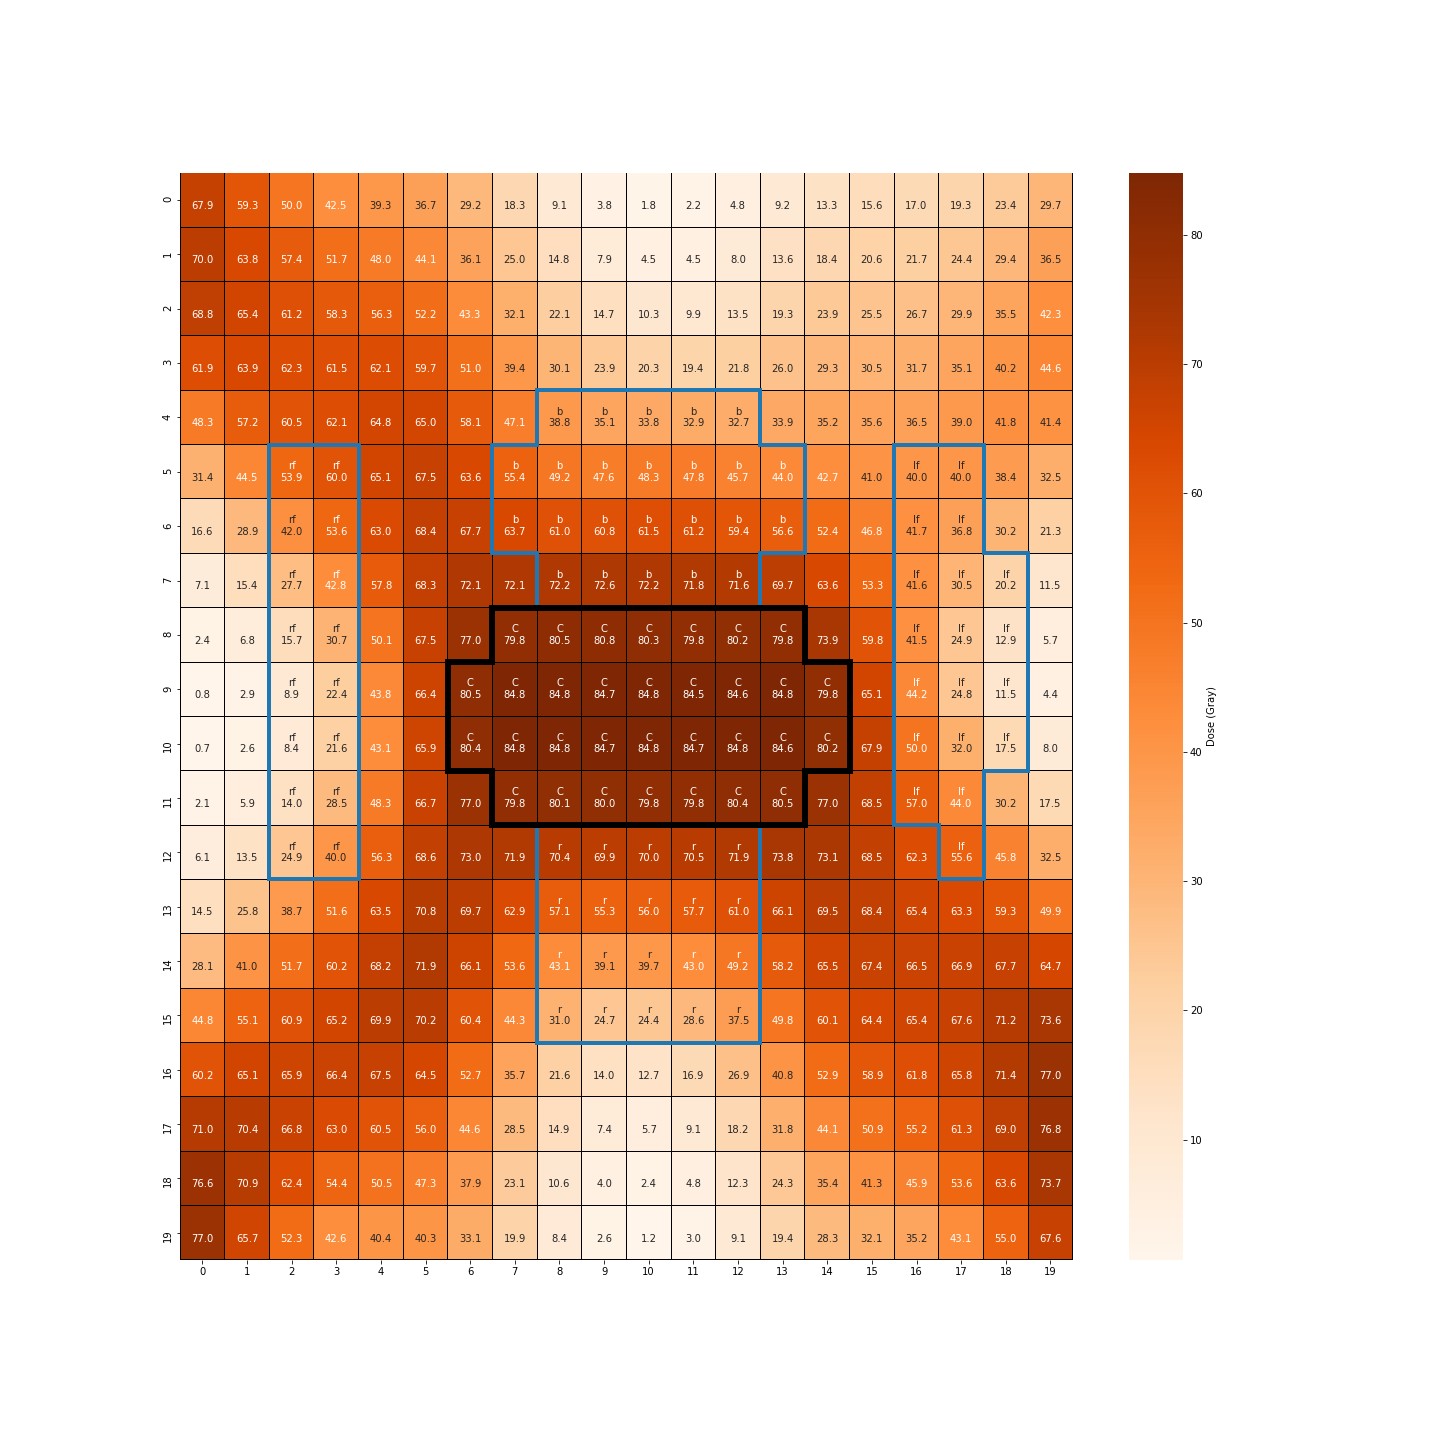
\includegraphics[width=0.95\columnwidth]{a-dose.png}
    \caption{Dose Distribution of Plan A}
    
\end{figure}

\subsubsection{3.1.2 Beamlet Intensity of A}
The following figure shows intensities of all beamlets from 1 to 60. To interpret this, each row of the plot means the 6 different angles of the beam, and the columns are the 10 beamlets in each angle. The solution is relatively sparse as some beamlets have high intensities while other are basically unused. This implies under this setting of constraints, some beamlets have much higher priority than others.
\begin{figure}[H]
    \centering
    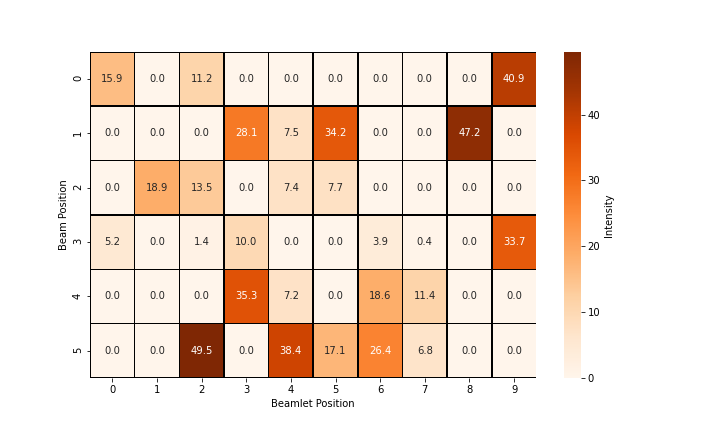
\includegraphics[width=0.6\columnwidth]{a-intensity.png}
    \caption{Beamlet Intensity of Plan A}
    
\end{figure}

\subsection{3.2 Plan B}

Compared to the Plan A, Plan B is less ``aggressive'' on the Bladder and Rectum, especially on the voxels that are connected to the CTV region. However, Plan B has higher radiation variance on the CTV region, and the Unspecified region may have ``overheated spot''. Similarly to Plan A, both Femur Heads are well protected as they are sensitive to the radiation. The objective is set to be minimizing the total doses received by all healthy regions (voxels that are not in the CTV region). That is:

\begin{center}
    $\min \sum_{j \notin \{\text{CTV}\}} D_j$
\end{center}
The following table shows the constraints set for this plan and the actual dose received by each region.

\begin{table}[H]
\centering
\begin{tabular}{||c|c c c||} 
 \hline
  & Actual Dose & Constraints & Ideal Constraints \\ [0.5ex] 
 \hline
 CTV Max & 85.8 & 85.8 & 84.8 \\ 
 CTV Min & 79 & 79 & 80.8 \\
 CTV Avg & 82.11 & - & 82.8 \\
 CTV Per & 8.21\% & 8.21\% & 5\% \\
 \hline
 Bladder Max & 75.51 & 81 & 81 \\
 Bladder Avg & 56.02 & 60 & 50 \\
 Bladder Per ($>$ 65) & 20.83\% & 22\% & 10\% \\ 
 \hline
 Rectum Max & 71.15 & 79.2 & 79.2 \\ 
 Rectum Avg & 45 & 45 & 40 \\ 
 \hline
 Unspecified Max & 83 & 83 & 72 \\ 
 \hline
 Left Femur Max& 48.86 & 55 & 50 \\ 
 Left Femur Per ($>$ 40)& 10.53\% & 15\% & 15\% \\ 
 \hline
 Right Femur Max& 47.30 & 55 & 50 \\ 
 Right Femur Per ($>$ 40)& 12.50\% & 15\% & 15\% \\ 
 \hline
\end{tabular}
\caption{Doses and Constraints of Plan B}
\label{table:2}
\end{table}

\subsubsection{3.2.1 Dose Distribution of B}

\begin{figure}[H]
    \centering
    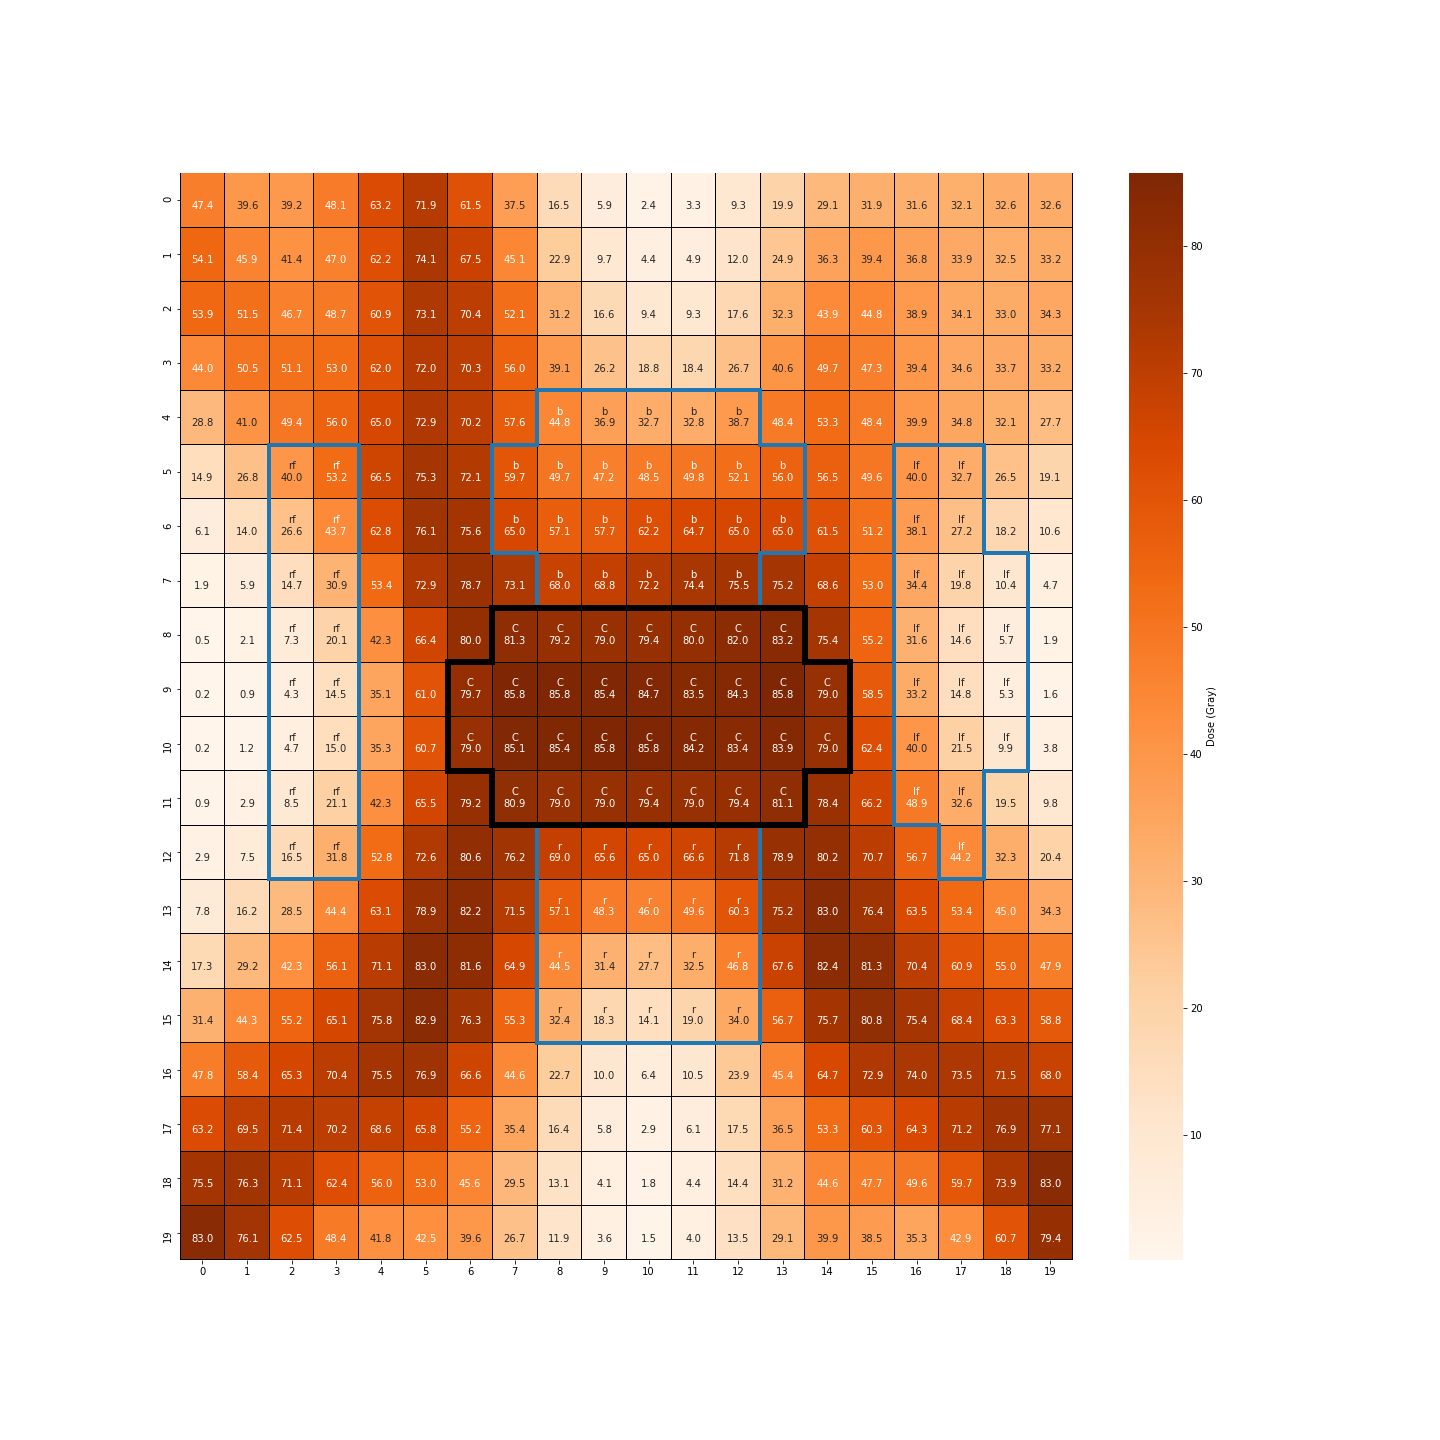
\includegraphics[width=0.95\columnwidth]{b-dose.png}
    \caption{Dose Distribution of Plan B}
    
\end{figure}

\subsubsection{3.2.2 Beamlet Intensity of B}

\begin{figure}[H]
    \centering
    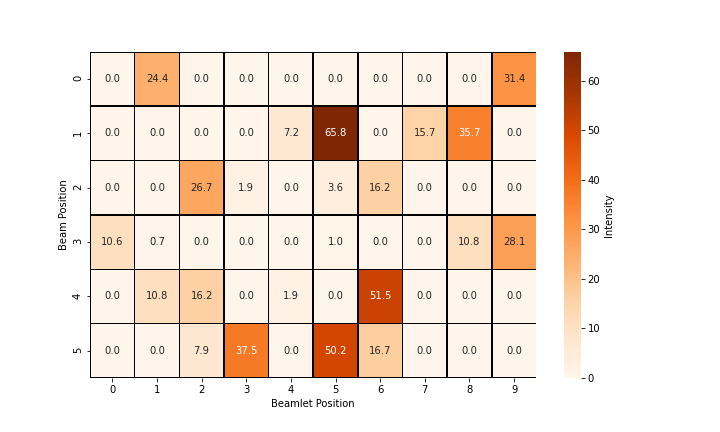
\includegraphics[width=0.6\columnwidth]{b-intensity.png}
    \caption{Dose Distribution of Plan B}
    
\end{figure}


\subsection{3.3 Plan C}
In order to avoid ``overheated spot'' in the Unspecified region,  we propose Plan C. Plan C delivers higher doses in the CTV region and Femur Heads but decreases the peak dose in the Unspecified region. Similar to Plan B, The objective is to set to be minimizing the total doses received by all healthy regions.
\begin{center}
    $\min \sum_{j \notin \{\text{CTV}\}} D_j$
\end{center}

The following table shows the constraints set for this plan and the actual dose received by each region.

\begin{table}[H]
\centering
\begin{tabular}{||c|c c c||} 
 \hline
  & Actual Dose & Constraints & Ideal Constraints \\ [0.5ex] 
 \hline
 CTV Max & 85.8 & 85.8 & 84.8 \\ 
 CTV Min & 79.8 & 79.8 & 80.8 \\
 CTV Avg & 82.12 & - & 82.8 \\
 CTV Per & 7.25\% & 7.25\% & 5\% \\
 \hline
 Bladder Max & 74.42 & 81 & 81 \\
 Bladder Avg & 57.00 & 57 & 50 \\
 Bladder Per ($>$ 65) & 25.00\% & 25\% & 10\% \\ 
 \hline
 Rectum Max & 72.44 & 79.2 & 79.2 \\ 
 Rectum Avg & 54.68 & 55 & 40 \\ 
 \hline
 Unspecified Max & 77 & 77 & 72 \\ 
 \hline
 Left Femur Max& 49.09 & 50 & 50 \\ 
 Left Femur Per ($>$ 40)& 10.53\% & 15\% & 15\% \\ 
 \hline
 Right Femur Max& 44.54 & 50 & 50 \\ 
 Right Femur Per ($>$ 40)& 12.50\% & 15\% & 15\% \\ 
 \hline
\end{tabular}
\caption{Doses and Constraints of Plan B}
\label{table:3}
\end{table}

\subsubsection{3.3.1 Dose Distribution of C}

\begin{figure}[H]
    \centering
    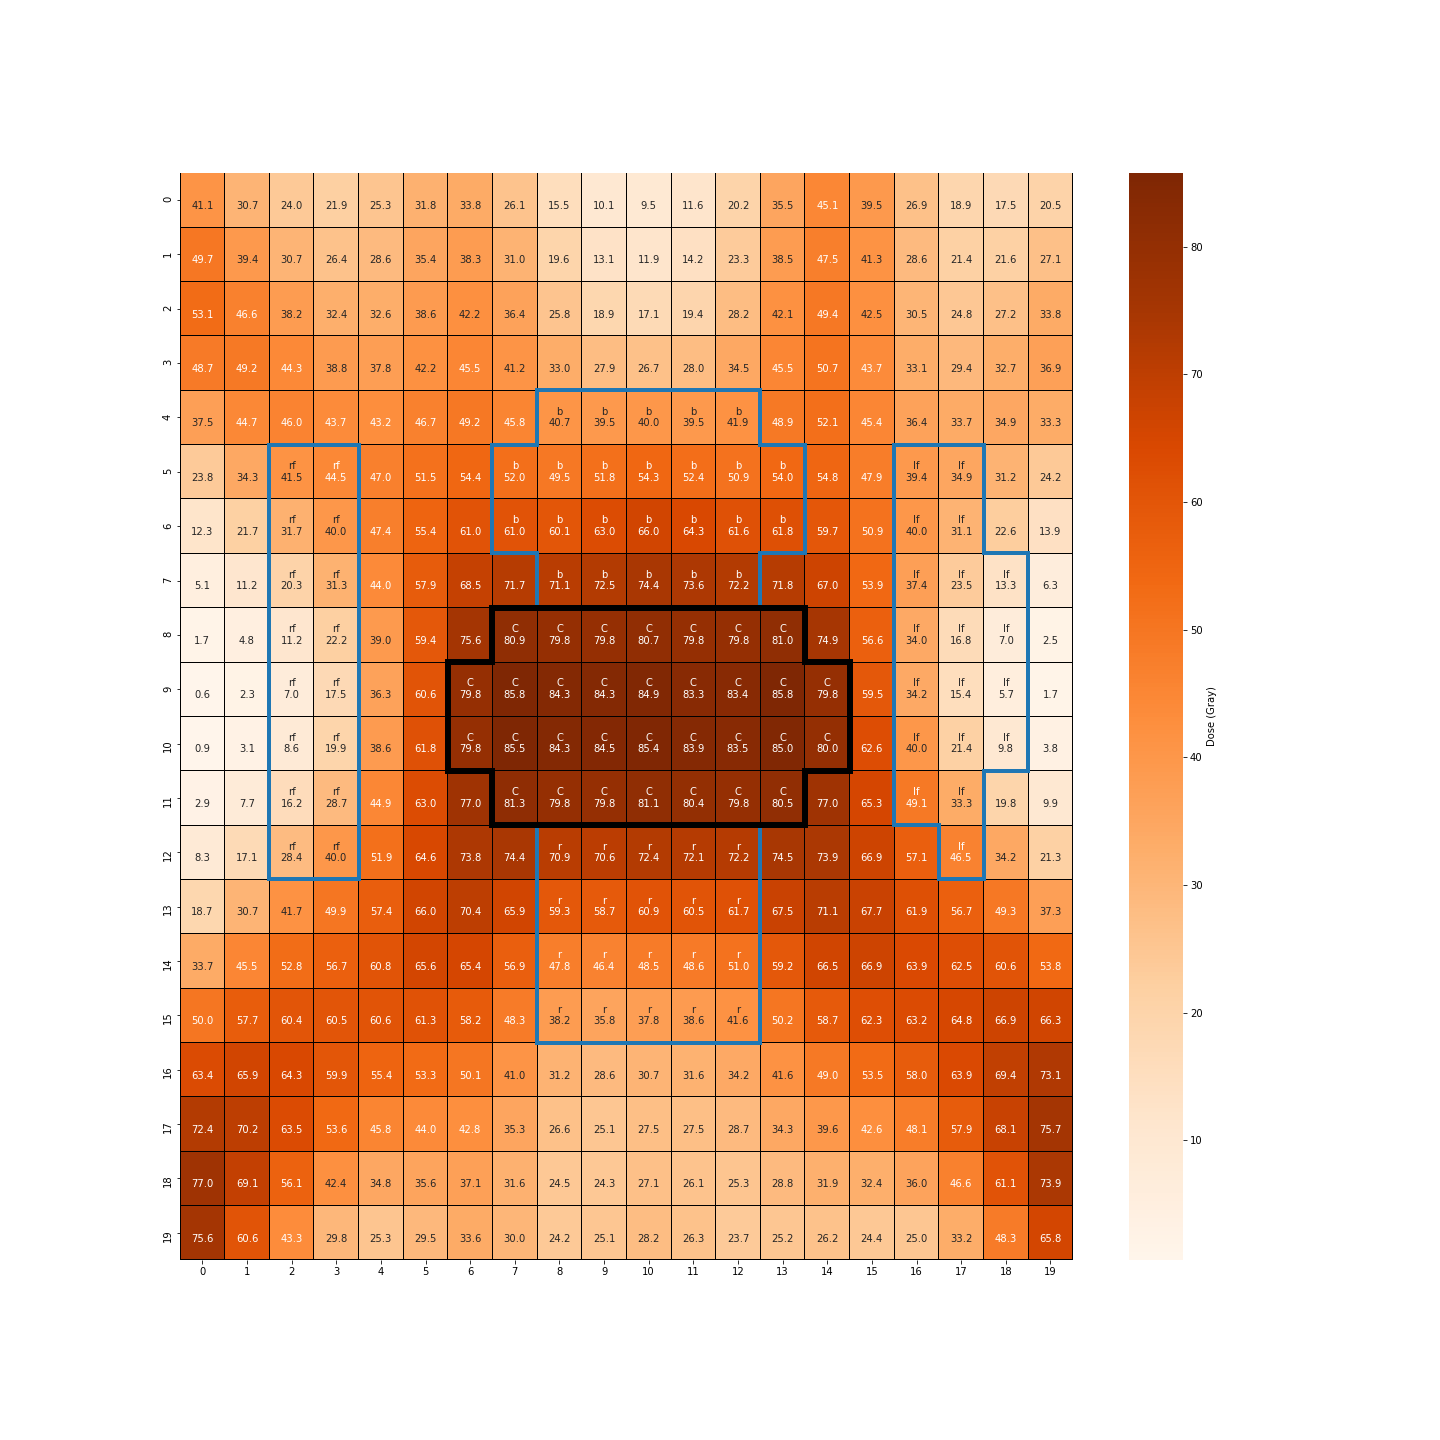
\includegraphics[width=0.95\columnwidth]{c-dose.png}
    \caption{Dose Distribution of Plan C}
    
\end{figure}

\subsubsection{3.3.2 Beamlet Intensity of C}

\begin{figure}[H]
    \centering
    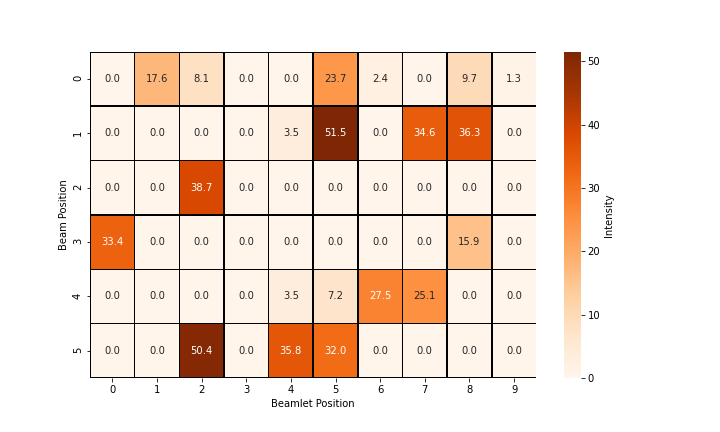
\includegraphics[width=0.6\columnwidth]{c-intensity.png}
    \caption{Beamlet Intensity of Plan C}
    
\end{figure}

\section{4. Conclusion}
We summarize 3 treatment plans we proposed. Every plan has pros and cons, so each plan may be targeted to a certain type of patients. Based on the optimization problems we solved, we can get a sense of how plans should be delivered.

\begin{table}[H]
    \centering
     \setlength{\leftmargini}{0.4cm}
    \begin{tabular}{| m{2cm} | m{4cm} | m{4cm} | m{4cm} |}
        \hline
        Name & Pros & Cons & Target Patients \\
        \hline
        Plan A & 
        \begin{itemize} 
            \item Uniform radiation in CTV without ``cold spot''
            \item Femur Heads are well protected
            \item Edges are highly radiated
            
        \end{itemize} & 
        \begin{itemize} 
            \item High radiation in Bladder and Rectum on average 
        \end{itemize} & 
        \begin{itemize} 
            \item Patients who seek the most effective plan

        \end{itemize} \\
        \hline
        Plan B & 
        \begin{itemize} 
            \item Lower radiation in Bladder and Rectum on average
            \item Femur Heads are well protected
        \end{itemize} & 
        \begin{itemize} 
            \item Some ``cold spots'' on the edge of CTV
            \item Peak radiation in the Unspecified region
            
        \end{itemize} & 
        \begin{itemize} 
            \item Patients who have sensitive Bladder or Rectum cells.  
        \end{itemize} \\
        \hline
        
        Plan C & 
        \begin{itemize} 
            \item Relatively uniform dose in CTV
            \item Low peak in the Unspecified region
            \item Femur Heads are well protected
        \end{itemize} & 
        \begin{itemize} 
            \item Relatively high radiation in Bladder and Rectum
            
        \end{itemize} & 
        \begin{itemize} 
            \item Patients who have sensitive cells in the Unspecified region.  
        \end{itemize} \\
        \hline
        
    \end{tabular}
\caption{Summary of 3 Plans}
\label{table:4}
\end{table}


\section{5. Discussion}

\subsection{5.1 Trade-off}
Based on the treatment plans we have, binding constraints are often among the ``Minimum CTV Dose'', ``Maximum CTV Dose'', ``Average Rectum Dose'' and ``Maximum Unspecified Dose''. Both Left Femur Head and Right Femur Head can usually be protected from high radiation. Maybe it`s due to the positions of organs of this patient. If we are given another input from a different patient, the binding constraints may vary. \\

Among the healthy organs, Bladder and Rectum are connected to the CTV region. In order to have a uniform radiation of tumor cells without ``cold spot'', they are likely to receive high doses. In all of these plans, Bladder and Rectum are overdosed on average, but we manage to avoid ``overheated spot''. If we are allowed to slack some of the constraints, we may slack ``Average Bladder Dose'' and ``Average Rectum Dose''.

\subsection{5.2 Variability}
The IMRT plans are delivered in fractions in multiple days, which introduces variations of positions of patients. In this project, we take care of this issue in two aspects:
\begin{itemize}
    \item In the classification of voxels, most voxels on the edges of the CTV region are classified as the CTV.
    \item In the plan A, we try to avoid ``cold spot'' and make the radiation more uniform in the CTV region. By doing this, voxels on the boundary are also highly radiated. But this may introduce some safety issues on the healthy organs nearby.
\end{itemize}

However, both approach assume the radiation are delivered uniformly each day. One possible approach is to give different plans in different days. We can define the ``core area'' and the ``edge area'' of the CTV region, and come up with different plans for different regions. Since the dose is accumulated, we can focus on the ``core area'' most of the days and take care of the ``edge area'' sometime.

\subsection{5.2 Other Approaches}
The non-linearity of integer programming increases the running time of the algorithm. In this 2D optimization program, we have 59 binary variables in total. If we solve the problem in a 3D space or use a finer grid, the number of binary variables will increase significantly.\\

Instead of formulating this optimization a linear programming problem, we can probably treat this problem as a general convex optimization and use gradient descent to find the optimum. The idea is to construct a loss function that penalizes overdoses or underdoses in all regions . And we can assign different weights to different regions to get different plans.


\section{6. Appendix}

\textbf{Solution A:}
[15.868387093681749, 0.0, 11.177228302249707, 0.0, 0.0, 0.0, 0.0, 0.0, 0.0, 40.91976141874853, 0.0, 0.0, 0.0, 28.091865730062302, 7.4874071119776, 34.15204155197002, 0.0, 0.0, 47.17733256643227, 0.0, 0.0, 18.8947209304184, 13.463645592256137, 0.0, 7.4011140440763565, 7.651046210069164, 0.0, 0.0, 0.0, 0.0, 5.197716439959529, 0.0, 1.429804646924821, 10.044500687093013, 0.0, 0.0, 3.9339655880369704, 0.3985800650851688, 0.0, 33.67009823297649, 0.0, 0.0, 0.0, 35.317475126183076, 7.2369777536785085, 0.0, 18.59593851359447, 11.402504940355886, 0.0, 0.0, 0.0, 0.0, 49.531412429384005, 0.0, 38.44589656715621, 17.06318883705735, 26.36388056882432, 6.802124917796154, 0.0, 0.0] \\

\textbf{Solution B:}
[0.0, 24.409343099299715, 0.0, 0.0, 0.0, 0.0, 0.0, 0.0, 0.0, 31.389018509085226, 0.0, 0.0, 0.0, 0.0, 7.196435447855121, 65.80228283004259, 0.0, 15.675279233664055, 35.68303433132794, 0.0, 0.0, 0.0, 26.679569500334193, 1.940489862954584, 0.0, 3.6276469318478264, 16.155952837462006, 0.0, 0.0, 0.0, 10.64712777928269, 0.6783840300994299, 0.0, 0.0, 0.0, 0.9932021042157287, 0.0, 0.0, 10.843586526530673, 28.106052242718988, 0.0, 10.772139530104322, 16.168601568431573, 0.0, 1.9117193954089555, 0.0, 51.51586825749159, 0.0, 0.0, 0.0, 0.0, 0.0, 7.9000777515995155, 37.50161333439625, 0.0, 50.24587812215735, 16.73690534456178, 0.0, 0.0, 0.0] \\

\textbf{Solution C:}
[0.0, 17.6016722277992, 8.080519055820973, 0.0, 0.0, 23.678625171394454, 2.3515025602153954, 0.0, 9.694832824917027, 1.3441278597710364, 0.0, 0.0, 0.0, 0.0, 3.5147238017073756, 51.491653160019844, 0.0, 34.578798733988044, 36.33815584426022, 0.0, 0.0, 0.0, 38.6647395604602, 0.0, 0.0, 0.0, 0.0, 0.0, 0.0, 0.0, 33.417963364567875, 0.0, 0.0, 0.0, 0.0, 0.0, 0.0, 0.0, 15.869790381419168, 0.0, 0.0, 0.0, 0.0, 0.0, 3.4966021256263975, 7.214833503315581, 27.501830231009205, 25.108439248684483, 0.0, 0.0, 0.0, 0.0, 50.440330083400475, 0.0, 35.76409349372485, 31.966958164836427, 0.0, 0.0, 0.0, 0.0]

\end{document}
